\section{Why filter after chaining but before alignment?}
\label{sec:prefilter-role}

The seed and chaining stages do not prove that two sequence intervals are
similar.  They prove only that a set of exact or hashed seed matches can be
arranged into a plausible region.  A repetitive target, a short seed, or a
noisy query can therefore produce regions whose base-level alignment is
hopeless.  Sending every such region to affine-gap dynamic programming is
correct, but it can be unnecessarily expensive: alignment must fill or
traverse a band, maintain several score states, and often retain enough state
for traceback.  A \emph{pre-alignment filter} is a cheaper decision procedure
inserted between candidate construction and dynamic programming.  Its useful
answer is not ``these strings align'', but ``this candidate cannot possibly
satisfy the requested edit threshold''.

This distinction is important in BioSeqDB because filtering is exposed through
an exact SQL predicate.  A query may ask for

\begin{verbatim}
WHERE mmsearch(seq, query)
  AND bioseq.edit(seq) < 10
\end{verbatim}

The SQL expression means that returned alignments have unit-cost edit distance
strictly below ten.  It does not mean that the database may return the
approximation computed by SneakySnake or GateKeeper.  The planner therefore
normalises the exclusive bound \(B=10\) to the inclusive prefilter threshold
\(E=B-1=9\).  A cheap stage may remove a candidate only when it can prove that
its distance is greater than \(E\).  Every survivor still undergoes the selected
base aligner, and an exact post-traceback stage applies the original strict
bound.  In current source this ordering is explicit in
\texttt{pipe.cppm}: the \texttt{PrefilterStage} is followed by
\texttt{AlignStage}, then \texttt{ExactEditFilterStage}, before the final
primary/secondary classification and mapping-quality calculation
(\texttt{pipe.cppm}, lines 8618--8628 in the inspected revision).

Let \(D(Q,T)\) denote the global unit-cost Levenshtein distance of a mandatory
query gap \(Q\) and target gap \(T\).  A conventional safe filter computes a
quantity \(L(Q,T)\) with
\[
        0 \le L(Q,T) \le D(Q,T).
\]
It rejects only if \(L(Q,T)>E\).  The two possible filter outputs are therefore
asymmetric:

\begin{center}
\begin{tabular}{p{0.20\textwidth}p{0.31\textwidth}p{0.39\textwidth}}
\textbf{Filter output} & \textbf{What is established} & \textbf{Pipeline action}\\
\hline
reject & the threshold cannot be met in the safe domain & omit expensive
alignment for this region\\
accept & nothing more than ``not disproved'' & align, reconstruct the exact
edit count, and enforce the SQL predicate\\
\end{tabular}
\end{center}

A false accept wastes time but does not change query results.  A false reject
removes a valid alignment and is a correctness error.  This is why the chapter
uses \emph{conservative accept} for unsupported geometry and why benchmark
tables report false rejects separately from throughput.

\subsection{The safe rejection domain in BioSeqDB}

The mapper does not globally align an entire chained region in one rectangular
problem.  Seeds already account for exact anchored pieces, while alignment
fills the gaps between successive seeds and may extend locally at the left and
right ends.  A lower bound for a mandatory seed-to-seed gap is composable:
disjoint mandatory gaps require disjoint edits, so their lower bounds may be
summed for a region.  A bound derived from a local extension window is not
composable in the same way.  X-drop or local alignment may legitimately omit
an expensive prefix or suffix; rejecting because that optional window has a
large global distance would delete a valid local result.

BioSeqDB therefore materialises only mandatory global fill windows.  The
iteration at \texttt{pipe.cppm}, lines 7985--8048, converts each window to flat
alphabet ranks, applies reverse-query orientation when required, and records
which region owns the job.  Left and right local extensions are deliberately
excluded.  Results are accumulated per region with saturating addition, and
stable in-place compaction retains survivor order (lines 8105--8162).  This is
narrower than applying a published filter to the whole candidate interval, but
it matches the semantic unit that the aligner is obliged to solve.

Three additional rules close common correctness gaps:

\begin{enumerate}
    \item For unequal-length windows, both implemented filters use only
    \(\lvert |Q|-|T| \rvert\), an exact lower bound on the number of
    insertions and deletions.  The equal-length chip-maze or bit-mask
    approximation is not extrapolated to geometry for which the port has no
    proof.
    \item Invalid, overflowing, or unsupported jobs return status
    \texttt{unsupported\_conservative} and are accepted.  ``Fail open'' here
    means preserving candidates, not ignoring an execution error.
    \item If a Vulkan backend was explicitly selected and its runtime or
    hardware execution fails, the query fails rather than silently changing to
    CPU.  This is a route-integrity rule.  It is distinct from the
    conservative-accept result returned for a representable unsupported job.
\end{enumerate}

The common ABI makes these cases visible.  \texttt{PrefilterJob} is a 20-byte
record containing two offsets, two lengths, and \(E\);
\texttt{PrefilterResult} is a 16-byte record containing a lower bound, status,
accept bit, and diagnostic word
(\texttt{prefilter\_types.cppm}, lines 16--61).  The three statuses are
\texttt{success}, \texttt{conservative\_unequal}, and
\texttt{unsupported\_conservative}.  The same records cross the scalar,
Highway, and Vulkan boundaries, avoiding a host-side translation whose
semantics could drift.

\subsection{Difference from the minimap2 baseline}

The minimap2 pipeline supplies the surrounding algorithm but not this
query-scoped filter.  After chaining and region selection, ordinary minimap2
invokes its KSW2 extension machinery for the selected candidate gaps and uses
alignment scores, z-drop, and traceback to decide how the region should be
reported.  It has seed-frequency and chaining heuristics that reduce the
candidate set, but these are not a proof of the SQL condition
\(\operatorname{edit}<B\).  The SneakySnake and GateKeeper papers likewise
evaluate candidate read/reference pairs before an exact aligner; neither
defines how an edit predicate should participate in PostgreSQL planning.

BioSeqDB preserves minimap2-derived seeds, chains, region geometry, and the
chosen final aligner.  It inserts one additional conditional stage after
divergence estimation and before base alignment.  The stage is enabled only
when the query requests exact edit accounting and provides a representable
positive strict bound.  Rejection removes KSW2 or Block-Aligner work; acceptance
does not change scoring parameters, z-drop, CIGAR construction, primary versus
secondary classification, or mapping quality.  The exact survivor stage runs
before the final classification pass so a candidate that violates the SQL
predicate cannot influence another survivor's metadata.

This placement also explains why the implementation filters seed-to-seed gaps
rather than the raw pair used by the standalone paper tools.  Minimap2 has
already fixed exact seed anchors and may use local end extension.  BioSeqDB
adapts each underlying algorithm to that decomposition instead of changing the
decomposition to resemble the paper benchmark.  The whole-pipeline evidence in
Section~\ref{sec:prefilter-results} therefore reports avoided KSW2 calls and
input-cell area, which are more informative for this port than a standalone
filter throughput number alone.

\section{SneakySnake: routing through a chip maze}
\label{sec:prefilter-sneakysnake}

The original paper, \emph{SneakySnake: A Fast and Accurate Universal Genome
Pre-Alignment Filter for CPUs, GPUs, and FPGAs}, reformulates approximate
string matching as a single-net-routing problem.  For equal-length strings of
length \(m\) and threshold \(E\), it considers a grid with \(m\) columns and
\(2E+1\) rows.  A row represents one relative diagonal
\(d\in[-E,E]\).  At column \(j\), the cell is free when the target symbol
matches the query symbol at the shifted coordinate and is an obstacle
otherwise:
\[
 Z_d(j) =
 \begin{cases}
 0, & 0\le j+d<m \text{ and } Q[j+d]=T[j],\\
 1, & \text{otherwise.}
 \end{cases}
\]
The paper describes rows as horizontal routing tracks and columns as vertical
routing tracks.  A horizontal run of zero cells followed by at most one
obstacle is an \emph{escape segment}.  At a checkpoint, the algorithm examines
all \(2E+1\) diagonals, takes the longest zero run, crosses its following
obstacle if one exists, and advances the checkpoint.  Reaching the right
boundary with at most \(E\) obstacles means that exact alignment is still
necessary; observing more than \(E\) obstacles permits rejection.

Figure~\ref{fig:prefilter-chip-maze} reconstructs this mechanism rather than
copying the paper artwork.  Its visual grammar follows the project figure
reconstruction reference: a white background, explicit row labels, black
obstacles, and one amber route.  The particular bits are illustrative; the
invariant is the movement from one checkpoint to the furthest available
horizontal segment.

\begin{figure}[htbp]
\centering
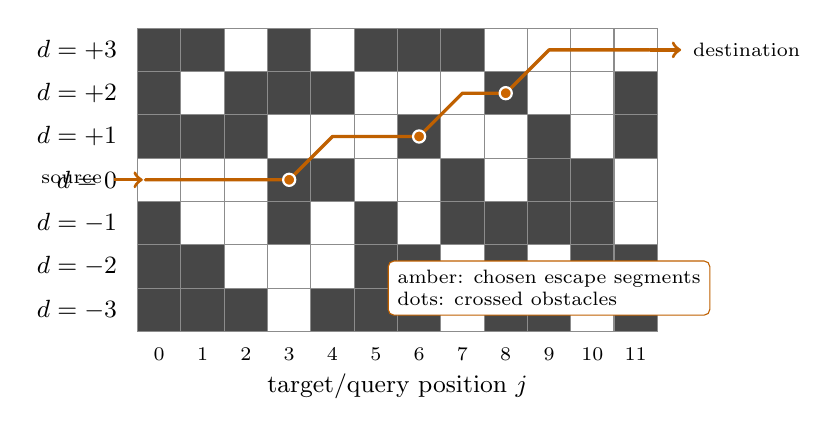
\begin{tikzpicture}[x=0.55cm,y=0.55cm,font=\small]
  \def\matchfill{white}
  \def\obstaclefill{black!72}
  \foreach \row/\lab/\bits in {
    6/{d=+3}/{1,1,0,1,0,1,1,1,0,0,0,0},
    5/{d=+2}/{1,0,1,1,1,0,0,0,1,0,0,1},
    4/{d=+1}/{1,1,1,0,0,0,1,0,0,1,0,1},
    3/{d=0}/{0,0,0,1,1,0,0,1,0,1,1,0},
    2/{d=-1}/{1,0,0,1,0,1,0,1,1,1,1,0},
    1/{d=-2}/{1,1,0,0,0,1,1,0,1,0,1,1},
    0/{d=-3}/{1,1,1,0,1,1,1,0,1,1,0,1}}
  {
    \node[anchor=east] at (-0.25,\row+0.5) {\(\lab\)};
    \foreach \b [count=\col from 0] in \bits {
      \ifnum\b=1
        \fill[\obstaclefill] (\col,\row) rectangle ++(1,1);
      \else
        \fill[\matchfill] (\col,\row) rectangle ++(1,1);
      \fi
      \draw[black!45,thin] (\col,\row) rectangle ++(1,1);
    }
  }
  \foreach \col in {0,...,11}
    \node[font=\scriptsize,anchor=north] at (\col+0.5,-0.15) {\col};
  \node[anchor=north] at (6,-0.75) {target/query position \(j\)};

  \draw[very thick,color=orange!75!black,line cap=round,line join=round]
    (0.18,3.5) -- (3.5,3.5) -- (4.5,4.5) -- (6.5,4.5)
    -- (7.5,5.5) -- (8.5,5.5) -- (9.5,6.5) -- (11.82,6.5);
  \foreach \x/\y in {3.5/3.5,6.5/4.5,8.5/5.5}
    \draw[fill=orange!80!black,draw=white,thick] (\x,\y) circle (0.14);
  \draw[->,very thick,color=orange!75!black] (-0.55,3.5) -- (0.12,3.5);
  \draw[->,very thick,color=orange!75!black] (11.82,6.5) -- (12.55,6.5);
  \node[anchor=east,font=\scriptsize] at (-0.6,3.5) {source};
  \node[anchor=west,font=\scriptsize] at (12.6,6.5) {destination};
  \node[draw=orange!75!black,fill=white,rounded corners=2pt,
        font=\scriptsize,align=left] at (9.5,1.0)
        {amber: chosen escape segments\\dots: crossed obstacles};
\end{tikzpicture}
\caption{Reconstruction of the SneakySnake chip-maze walk.  Each row is
a query--target shift, a white cell is a match, and a dark cell is an
obstacle.  From each checkpoint the route takes the longest immediately
available horizontal match run.  The number of crossed obstacles is used as
an edit-distance lower bound; the route does not reconstruct an edit script.}
\label{fig:prefilter-chip-maze}
\end{figure}

\subsection{Why the obstacle count can filter}

The chip maze is intentionally less expressive than dynamic programming.  It
does not charge vertical distance between escape segments and it does not
record which insertion, deletion, or substitution produced a shift.  That
loss of information is useful only in one direction: the route may
\emph{underestimate} the true edit distance, but a reliable implementation
must not overestimate it.  If the route crosses \(r\) obstacles and
\(r>D(Q,T)\), then a valid pair could be rejected.  The paper's central
argument is that the greedy route minimises obstacles in its routing model and
that this number is a lower bound for the corresponding equal-length global
matching problem.

In executable form, the core walk is:

\begin{verbatim}
lower_bound = 0
for each non-overlapping submaze [start,end):
    checkpoint = start
    while checkpoint < end:
        best = longest matching prefix among shifts -E..+E
        if best reaches end:
            break
        lower_bound += 1                  # cross one obstacle
        if lower_bound > E:
            reject
        checkpoint += best + 1
accept for exact alignment
\end{verbatim}

The current BioSeqDB scalar and Highway implementations follow this structure
in \texttt{sneaky\_snake.cppm}, lines 350--400.  The production submaze width
is 512 symbols.  Partitioning a long maze makes execution and GPU resource
requirements bounded; it can reduce filter strength by producing a smaller
lower bound, but that direction creates false accepts rather than false
rejects.

\subsection{From the reference implementation to the BioSeqDB port}

The checked-in reference scalar code operates on character arrays, loops over
DNA-like strings, partitions by a caller-provided \texttt{KmerSize}, and uses
labels to leave a diagonal scan at its first mismatch.  Its CUDA counterpart
uses fixed packing and compile-time dimensions.  BioSeqDB retains the
algorithmic walk but changes the representation and execution contract:

\begin{enumerate}
    \item \textbf{Alphabet-generic ranks.}  The filter compares normalised
    rank bytes for equality.  It does not encode \(A,C,G,T\) inside the
    algorithm, so DNA4, DNA5, amino-acid, and generated alphabets use the same
    primitive once the pipeline has materialised the mandatory gaps.  Equal
    numeric ranks are compared only after the surrounding sequence type has
    established a common alphabet.
    \item \textbf{Checked flat batches.}  Each job names slices in two flat
    rank arrays.  Offset and length checks occur before a load.  Oversized
    spans and invalid slices conservatively survive.
    \item \textbf{Safe unequal lengths.}  Instead of importing the archived
    unequal-maze deduction, the implementation returns the exact length
    difference and marks the result \texttt{conservative\_unequal}
    (\texttt{sneaky\_snake.cppm}, lines 402--425).
    \item \textbf{Pipeline-safe windows.}  Only mandatory global fills are
    evaluated.  Reverse-strand gaps are materialised in their oriented rank
    order.  Local extension regions never cause a rejection.
    \item \textbf{Query-scoped threshold.}  \(E\) is derived from the SQL
    predicate, not from a global feature switch.  The same query also enables
    exact edit accounting after alignment.
\end{enumerate}

The first CPU port performed one rank comparison at a time and the first SIMD
design vectorised several independent jobs with gather-heavy state.  That
implementation was correct but slower than the bundled C reference in most
standalone cells.  The retained scalar path now scans a matching prefix with
unaligned 64-bit loads, XOR, and first-differing-byte detection
(\texttt{sneaky\_snake.cppm}, lines 74--154).  The retained Highway path loads
contiguous rank bytes, compares complete vectors, and locates the first true
mismatch lane (lines 156--214).  At a checkpoint, the implementation first
measures the unshifted diagonal, freezes the best length, and tests a candidate
shift only if the query symbol at that best-offset could improve the result.
Highway applies this candidate test to a contiguous window, avoiding the
earlier per-lane job-state machinery (lines 263--348).

The optimisation is exact, not heuristic.  Suppose the current best run has
length \(b\).  A candidate diagonal can improve the maximum only if its first
\(b\) symbols match; in particular, it must match the target at offset \(b\).
Testing that symbol discards only candidates that cannot beat the current
best.  Full prefix scanning is performed for every surviving candidate.

\subsection{SneakySnake on Vulkan}

The Vulkan route uses the same job and result layout as the CPU paths and one
hardware-only runtime.  The shader domain is bounded by a 512-symbol submaze
and \(E\le31\) (\texttt{phase\_c\_abi.cppm}, lines 61--64).  Larger thresholds
return an unsupported conservative result.  Two execution modes were retained
after measurement:

\begin{itemize}
    \item mode 1 assigns an independent invocation to a job and is used for
    low thresholds, where synchronisation and team setup cost more than they
    save;
    \item mode 8 uses an eight-lane team when at least one supported
    equal-length job has \(E\ge16\), exposing diagonal work in parallel.
\end{itemize}

The resolver is visible at \texttt{runtime.cppm}, lines 14939--14975.  Both
modes have persistent recorded-command identities.  Descriptor bindings,
push bytes, group count, and pipeline identity are part of the replay key, so
reusing a command buffer cannot replay stale geometry.  Rank buffers,
descriptor state, memory-admission accounting, fences, and result storage are
shared with GateKeeper rather than duplicated.  A hardware support probe never
turns software Vulkan such as llvmpipe into a claimed GPU result.

\section{GateKeeper: shifted masks, amendment, and an exact guard}
\label{sec:prefilter-gatekeeper}

SneakySnake is attractive over a wide range of lengths and thresholds, but its
checkpoint loop and diagonal scans leave fixed overhead for very small seed
gaps.  GateKeeper is a bit-vector filter derived from Shifted Hamming Distance.
The original GateKeeper-GPU system packs DNA symbols into two bits, creates one
CUDA thread per read/reference pair, and fixes read length and threshold at
compile time.  Its small, regular boolean data flow is a better match for the
32- and 64-symbol gaps that occur in the BioSeqDB pipeline.

For equal-length \(Q,T\) and threshold \(E\), define a mismatch mask on the
unshifted diagonal,
\[
 H_0[j] = [Q[j]\ne T[j]],
\]
and two masks for every displacement \(d=1,\ldots,E\):
\[
\begin{split}
 H_{-d}[j] &= [j\ge d \ \land\ Q[j-d]\ne T[j]],\\
 H_{+d}[j] &= [j+d<m \ \land\ Q[j+d]\ne T[j]].
\end{split}
\]
Thus the filter constructs \(2E+1\) logical masks.  A zero in a mask denotes a
possible match.  Insertions and deletions move a true match run away from the
main diagonal, so the shifted rows can expose it.

\subsection{Why masks are amended}

A single accidental zero dominates a bitwise AND even if all other diagonals
contain mismatches at that position.  GateKeeper therefore \emph{amends}
short internal runs of zeros before combining masks.  In the BioSeqDB
clean-room implementation, a zero run is filled only when it is bounded by
ones and has length one or two.  Edge runs and runs of three or more are
preserved.  For a conceptually unbounded bit vector \(M\), with zeros outside
the valid sequence interval, the operation can be expressed as
\[
\begin{split}
\mathrm{single} &=
   \neg M \land (M\ll1) \land (M\gg1),\\
\mathrm{pairStart} &=
   \neg M \land (\neg M\gg1) \land (M\ll1) \land (M\gg2),\\
\mathrm{amend}(M) &=
   M \lor \mathrm{single} \lor \mathrm{pairStart}
      \lor (\mathrm{pairStart}\ll1).
\end{split}
\]
The result is masked back to valid positions.  Multiword implementations must
carry neighbouring bits across 32-bit boundaries; otherwise a two-zero run
straddling a word boundary would be treated differently from the same pattern
inside a word.

Shifting introduces vacant edge positions.  Leaving them as zero would let the
final AND hide a leading or trailing error.  Following the GateKeeper-GPU
improvement, BioSeqDB amends the shifted mask first and then marks the newly
exposed boundary as a mismatch:
\[
 \mathrm{amend}(H_{-d})[d-1]\gets1,\qquad
 \mathrm{amend}(H_{+d})[m-d]\gets1.
\]
The ordering matters.  Applying compensation before amendment could cause the
new boundary one to fill an adjacent edge run and change the intended mask.

All amended masks are ANDed.  The resulting bit vector is divided into
four-bit groups.  A zero nibble costs zero.  The patterns
\[
 0101,\ 0110,\ 1001,\ 1010,\ 1011,\ 1101
\]
cost two, and every other nonzero nibble costs one.  Accumulation stops at
\(E+1\).  This reproduces the reference cost semantics without importing its
16-entry CUDA lookup table.

Figure~\ref{fig:prefilter-gatekeeper} reconstructs the data flow from the
original paper and kernel.  It emphasises a feature that is easy to miss in a
prose description: amendment is performed per shifted mask \emph{before} the
mask intersection, and the final count is a grouped estimate rather than a
popcount.

\begin{figure}[htbp]
\centering
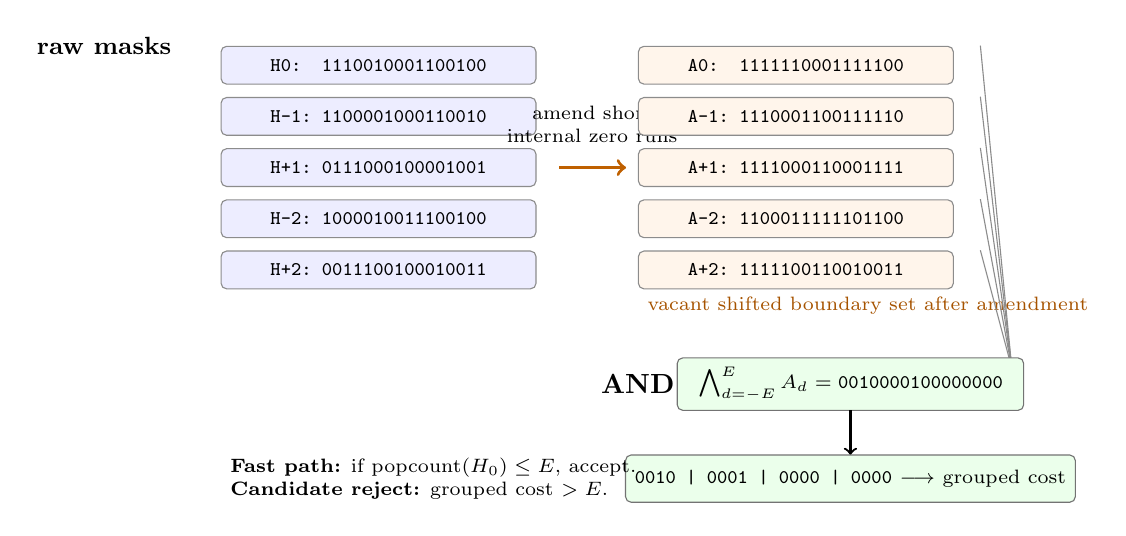
\begin{tikzpicture}[x=1cm,y=1cm,font=\scriptsize]
  \node[anchor=east,font=\small\bfseries] at (1.5,5.45) {raw masks};
  \node[anchor=west,draw=black!45,fill=blue!7,rounded corners=2pt,
        minimum width=4.0cm,minimum height=0.48cm] at (2,5.2)
        {\texttt{H0:\ \ 1110010001100100}};
  \node[anchor=west,draw=black!45,fill=blue!7,rounded corners=2pt,
        minimum width=4.0cm,minimum height=0.48cm] at (2,4.55)
        {\texttt{H-1:\ 1100001000110010}};
  \node[anchor=west,draw=black!45,fill=blue!7,rounded corners=2pt,
        minimum width=4.0cm,minimum height=0.48cm] at (2,3.90)
        {\texttt{H+1:\ 0111000100001001}};
  \node[anchor=west,draw=black!45,fill=blue!7,rounded corners=2pt,
        minimum width=4.0cm,minimum height=0.48cm] at (2,3.25)
        {\texttt{H-2:\ 1000010011100100}};
  \node[anchor=west,draw=black!45,fill=blue!7,rounded corners=2pt,
        minimum width=4.0cm,minimum height=0.48cm] at (2,2.60)
        {\texttt{H+2:\ 0011100100010011}};

  \draw[->,very thick,color=orange!75!black] (6.3,3.9) -- (7.15,3.9);
  \node[align=center,font=\scriptsize] at (6.72,4.45)
        {amend short\\internal zero runs};

  \node[anchor=west,draw=black!45,fill=orange!8,rounded corners=2pt,
        minimum width=4.0cm,minimum height=0.48cm] at (7.3,5.2)
        {\texttt{A0:\ \ 1111110001111100}};
  \node[anchor=west,draw=black!45,fill=orange!8,rounded corners=2pt,
        minimum width=4.0cm,minimum height=0.48cm] at (7.3,4.55)
        {\texttt{A-1:\ 1110001100111110}};
  \node[anchor=west,draw=black!45,fill=orange!8,rounded corners=2pt,
        minimum width=4.0cm,minimum height=0.48cm] at (7.3,3.90)
        {\texttt{A+1:\ 1111000110001111}};
  \node[anchor=west,draw=black!45,fill=orange!8,rounded corners=2pt,
        minimum width=4.0cm,minimum height=0.48cm] at (7.3,3.25)
        {\texttt{A-2:\ 1100011111101100}};
  \node[anchor=west,draw=black!45,fill=orange!8,rounded corners=2pt,
        minimum width=4.0cm,minimum height=0.48cm] at (7.3,2.60)
        {\texttt{A+2:\ 1111100110010011}};
  \node[anchor=west,font=\scriptsize,color=orange!65!black] at (7.3,2.15)
        {vacant shifted boundary set after amendment};

  \foreach \yy in {2.85,3.5,4.15,4.8,5.45}
    \draw[black!45] (11.65,\yy) -- (12.05,1.35);
  \node[draw=black!55,fill=green!8,rounded corners=2pt,
        minimum width=4.4cm,minimum height=0.60cm] at (10.0,1.15)
        {\(\bigwedge_{d=-E}^{E} A_d =
        \texttt{0010000100000000}\)};
  \node[font=\bfseries] at (7.3,1.15) {AND};
  \draw[->,thick] (10.0,0.82) -- (10.0,0.25);
  \node[draw=black!55,fill=green!8,rounded corners=2pt,
        minimum width=5.4cm,minimum height=0.60cm] at (10.0,-0.05)
        {\texttt{0010 | 0001 | 0000 | 0000}
         \(\longrightarrow\) grouped cost};
  \node[anchor=west,align=left] at (2,-0.05)
        {\textbf{Fast path:} if \(\mathrm{popcount}(H_0)\le E\), accept.\\
         \textbf{Candidate reject:} grouped cost \(>E\).};
\end{tikzpicture}
\caption{Reconstructed GateKeeper mask flow for \(E=2\).  Shifted Hamming
masks are amended independently, their vacant boundaries are compensated,
and all \(2E+1\) masks are intersected.  Four-bit groups of the final mask
produce a threshold estimate.  The strings are explanatory masks rather than
a reproduced experimental pair.}
\label{fig:prefilter-gatekeeper}
\end{figure}

\subsection{The exact guard changes the correctness argument}

The GateKeeper-GPU paper reports empirical filtering accuracy, including its
false-reject measurements, but an empirical zero is not a proof that every
possible input is safe.  Moreover, mask amendment deliberately changes match
bits to mismatch bits.  BioSeqDB therefore does not use the mask estimate alone
as a rejection proof.

The current scalar algorithm at \texttt{gatekeeper.cppm}, lines 178--279,
implements the following decision:

\begin{verbatim}
H = unshifted mismatch mask
if popcount(H) <= E:
    accept
if E == 0:
    reject                         # unequal symbols prove D > 0
A = amend(H)
for d = 1..E:
    A &= compensate(amend(H[-d]))
    A &= compensate(amend(H[+d]))
estimate = grouped_four_bit_cost(A), capped at E+1
if estimate <= E:
    accept
if exact_banded_Levenshtein(Q,T,E) says D > E:
    reject
accept                             # mask candidate was not exact
\end{verbatim}

Only a mask \emph{candidate} that is confirmed by exact thresholded global
Levenshtein distance becomes a rejection.  The banded predicate uses
\(2E+3\) cells per row, saturates values at \(E+1\), and for \(E\le8\) stores
two fixed 19-cell rows on the stack
(\texttt{edit\_distance\_threshold.cppm}, lines 99--159).  Its time is
\(O(mE)\), but it runs only on pairs that the much cheaper mask wants to
reject.  The four measured fixed Vulkan shaders use an equivalent bounded
wavefront guard and reuse mismatch masks for longest-common-prefix extension.

This design gives a stronger guarantee than the published heuristic alone:
a mask false reject is converted to an accept by the exact guard.  It also
changes the meaning of the result fields.  A GateKeeper mask acceptance
contributes numeric lower bound zero.  A confirmed rejection returns \(E+1\).
The raw mask estimate is diagnostic and must not be summed across region gaps.
Four bits in the result word identify a mask-rejection candidate, guard
activation, guard-confirmed rejection, or the exact \(E=0\) Hamming rejection
(\texttt{prefilter\_types.cppm}, lines 63--78 and 128--155).

\subsection{Clean-room, alphabet-generic implementation}

The reference CUDA kernel has several properties that are unsuitable as a
database extension boundary.  It encodes only \(A,C,G,T\) in two bits; passes
undefined symbols by a separate rule; allocates a compile-time
\((2E+1)\)-by-word mask matrix per thread; performs explicit carry repair
between 32-bit words; uses a constant-memory amendment lookup table; and
requires recompilation when length or threshold changes.  Host orchestration
uses CUDA unified memory and mapper-specific batches.

BioSeqDB re-derived the operations over equality-comparable rank bytes.  The
CPU oracle uses a 128-bit logical mask, with direct support for equal nonempty
lengths up to 128 and \(E\le8\)
(\texttt{gatekeeper.cppm}, lines 21--26 and 164--172).  It preserves short
internal zero-run semantics using shifts rather than importing the lookup
table.  DNA rank zero has no special interpretation, and the same code works
for DNA5 or amino-acid ranks because a shifted vacant cell is represented by a
mask boundary rule, not by a fake alphabet symbol.

The Vulkan implementation consists of one generic shader plus four fixed
production variants:
\[
 (m,E)\in\{(32,2),(32,4),(64,2),(64,4)\}.
\]
All have local size 64 and maximum span 128; the static variant registry is
explicit in \texttt{shader\_variants.cppm}, lines 344--353.  A fixed variant is
chosen only for a homogeneous batch whose rank offsets are four-byte aligned.
It loads the packed rank words once, derives Hamming and shifted masks in
registers, retains only the raw diagonals needed by its pruned exact
wavefront, and does not reread rank storage during the guard.  Any other direct
GateKeeper batch uses the generic shader.  The production pipeline is even
narrower: automatic GateKeeper selection requires every job to have length 32
or 64 and threshold 2 or 4.

\begin{table}[htbp]
\centering
\small
\begin{tabular}{p{0.20\textwidth}p{0.34\textwidth}p{0.36\textwidth}}
\textbf{Property} & \textbf{GateKeeper-GPU reference} & \textbf{BioSeqDB GateKeeper}\\
\hline
Input symbols & two-bit DNA; undefined base handled specially &
alphabet-normalised rank equality; no DNA constant in the algorithm\\
Execution API & CUDA kernel, one pair per thread, compile-time \(m,E\) &
shared batch ABI; Vulkan generic shader plus four measured fixed variants\\
Mask storage & \(2E+1\) word arrays per thread &
streamed/intersected masks; fixed variants keep packed ranks and required
diagonals in registers\\
Amendment & 16-entry LUT plus cross-word repair &
boolean run definition, explicitly tested at word boundaries\\
Shift boundary & leading/trailing OR compensation &
same semantic compensation, applied after amendment and valid-bit masking\\
Rejection basis & approximate grouped mask count &
mask candidate plus exact bounded global-edit guard\\
Unsupported input & mapper-specific handling &
status-2 conservative accept; selected runtime failure remains an error\\
\end{tabular}
\caption{Algorithmic and systems differences between the research
GateKeeper-GPU implementation and the BioSeqDB port.}
\label{tab:gatekeeper-differences}
\end{table}

\section{Dispatch and integration with the query pipeline}
\label{sec:prefilter-dispatch}

Algorithm choice and backend choice are related but not identical.  Scalar and
Highway production always use SneakySnake.  A Vulkan batch is resolved as
GateKeeper only when \emph{every} job belongs to the measured small-window
domain; otherwise the whole batch uses SneakySnake.  The pure resolver at
\texttt{pipe.cppm}, lines 7912--7934, is equivalent to:

\begin{verbatim}
if backend != Vulkan:
    return SneakySnake
if jobs is nonempty and
   every job has equal length in {32,64} and E in {2,4}:
    return GateKeeper
return SneakySnake
\end{verbatim}

Batch-wide resolution avoids two uploads, two queue submissions, and a result
merge.  It also makes the selected algorithm visible in execution proof.
Direct GateKeeper tests may exercise lengths through 128 and thresholds through
8, but that larger correctness domain is not automatically promoted to
production.  Performance evidence, not mere functional support, controls the
AUTO domain.

At the PostgreSQL boundary, the planner accepts exactly one top-level
\texttt{bioseq.edit(sequence\_column) < integer\_constant} predicate using the
built-in operators for 16-, 32-, or 64-bit integer constants.  An overloaded
operator merely named ``\(<\)'', a nonconstant bound, a wrong target column,
\(\le\), or an ambiguous placeholder does not enter the optimisation
(\texttt{custom\_scan.cppm}, lines 1976--2050).  Unsupported forms fail with a
feature-not-supported error rather than silently evaluating a stub with
different semantics.

When the strict predicate is active and \(B>0\) fits the prefilter ABI, the
custom scan sets \(E=B-1\).  Backend selection then follows current execution
capability:

\begin{itemize}
    \item an existing Vulkan minimisation, seeding, chaining, or extension
    route selects Vulkan for the prefilter too;
    \item a per-call
    \texttt{aligner\_options(vulkan\_enabled => true)} may explicitly request
    the standalone Vulkan prefilter;
    \item otherwise the scan selects Highway when vectorisation is enabled and
    scalar when it is disabled.
\end{itemize}

The global Vulkan capability flag alone does not unexpectedly move a scalar
query to the GPU.  This logic is visible at
\texttt{custom\_scan.cppm}, lines 23383--23414.  Negative or zero exclusive
bounds still reach the exact post-alignment predicate, but do not manufacture
an unsigned prefilter threshold.

The seven persistent command-replay routes make the heterogeneous data plane
explicit: SneakySnake mode 1, SneakySnake mode 8, generic GateKeeper, and the
four fixed GateKeeper variants.  \texttt{runtime.cppm}, lines 136--223, maps
each shader/push-mode combination to a distinct slot.  Both algorithms reuse
one admitted high-water workspace and descriptor cache.  Result validation
checks not just output count but status, threshold bounds, algorithm-specific
diagnostic bits, and the relationship between rejection and guard counters.

An \texttt{EXPLAIN ANALYZE} proof can consequently distinguish capability from
actual work.  The final GateKeeper SQL run recorded:
\texttt{algorithm: batch\_resolved\_gatekeeper\_or\_sneaky\_snake},
\texttt{Prefilter Resolved Algorithm: gatekeeper}, three Vulkan dispatches,
three evaluated jobs, one rejected region, one mask candidate, one guard
activation, and one guard-confirmed rejection.  The following exact stage
retained two rows with edit counts zero and four under the strict bound five.

\section{Intermediate results and the final routing policy}
\label{sec:prefilter-results}

The performance history matters because the final policy was not obvious from
the papers.  A fast published filter can become slower after generic rank
conversion, safe bounds checks, batching, runtime validation, and GPU
synchronisation are included.  The project benchmark therefore measures
\texttt{backend\_batch\_ns}: upload, dispatch, synchronisation, and result
readback are inside the timed region.  Correctness preparation and the exact
truth oracle are outside it.

\subsection{The first SneakySnake port: correct but usually slower}

The final-source intermediate run
\texttt{main/reporting/bioseq\_bench/report\_127.json} was produced on
2026-07-16 with
\texttt{meta.commit=679aa4264853eeaaa8a3bd2c891e8e2da7e8e967},
\texttt{dirty=true}, and \texttt{fast=false}.  The implementation report
attributes the dirty flag to local builder configuration and an untracked
generated report and states that compiled source matched the pushed commit;
the artefact is consequently described as a scoped measurement, not as a
clean-tree run.  Each standalone cell used a
deterministic 1,024-pair prefix from the bundled upstream corpus.  Decisions
matched the original and false rejects were zero, but Table
\ref{tab:sneaky-intermediate} shows that the initial BioSeqDB SIMD path was
between \(2.39\times\) and \(2.85\times\) the original kernel time.

\begin{table}[htbp]
\centering
\small
\begin{tabular}{lrrrr}
\textbf{Fixture/threshold} & \textbf{Original} & \textbf{Scalar} &
\textbf{Highway} & \textbf{Highway/original}\\
\hline
ERR, 100 bp, \(E=2\)   & 0.144 ms & 0.137 ms & 0.343 ms & 2.386\\
SRR, 250 bp, \(E=8\)   & 0.919 ms & 1.255 ms & 2.375 ms & 2.585\\
ERR, 100 bp, \(E=40\)  & 9.471 ms & 12.731 ms & 27.015 ms & 2.852\\
SRR, 250 bp, \(E=100\) & 58.331 ms & 87.035 ms & 161.071 ms & 2.761\\
\end{tabular}
\caption{Intermediate SneakySnake standalone P50 results from report 127.
All rows had identical decisions and zero false rejects.  The table explains
why the first SIMD design was not accepted as the final kernel.}
\label{tab:sneaky-intermediate}
\end{table}

Even a slower filter can improve an end-to-end mapper if it removes enough
alignment work.  The same report measured the complete candidate pipeline:

\begin{table}[htbp]
\centering
\small
\begin{tabular}{lrrrp{0.30\textwidth}}
\textbf{Fixture} & \textbf{Off} & \textbf{Scalar} & \textbf{Highway} &
\textbf{Observed downstream work}\\
\hline
MEDIUM\_HIFI & 22.145 ms & 22.193 ms & 22.309 ms &
no region rejected; 175 KSW2 calls and 6,672,027 input cells in every row\\
MEDIUM\_ONT\_MODERN & 21.864 ms & 10.646 ms & 10.373 ms &
all six candidate regions removed; KSW2 calls \(160\to0\), input cells
\(6{,}915{,}415\to0\)\\
\end{tabular}
\caption{Whole-pipeline P50 results from report 127.  Threshold-qualified
truth/correct counts matched the no-prefilter row.}
\label{tab:sneaky-pipeline}
\end{table}

The HiFi case is the break-even warning: if a filter rejects nothing, its work
is pure overhead and the result is neutral or slightly slower.  The ONT
fixture is the intended case: avoiding dynamic programming more than repays
the filter and produces approximately \(2.1\times\) speedup.  The ONT exact
threshold truth set was empty, so ``recall one'' there is vacuous; parity is
instead established by the independently computed truth/correct counts and
unchanged empty match result.

\subsection{Optimised SneakySnake CPU and Vulkan}

The next-day optimisation replaced gather-heavy independent-job SIMD with the
contiguous-byte traversal described earlier, added the frozen-best candidate
test, introduced the hybrid Vulkan mode, and retained recorded commands.
DOC0382 identifies report 138 as the final uncontended reproduction:

\begin{center}
\begin{tabular}{p{0.30\textwidth}p{0.23\textwidth}p{0.35\textwidth}}
\textbf{Comparison in report 138} & \textbf{Ratio to bundled original CPU} &
\textbf{Interpretation}\\
\hline
production Highway, equal-weight mean over cells & 0.708 &
29.2\% faster across the configured matrix\\
production Highway, summed P50 & 0.482 &
51.8\% less summed kernel time\\
Vulkan, summed P50 & 0.175 &
82.5\% less summed time; \(5.73\times\) throughput\\
\end{tabular}
\end{center}

All final Vulkan cells reported an available backend, 1,024 evaluated jobs,
valid result count, runtime validation, zero reference-decision mismatches, and
zero false rejects.  Command replay reduced summed GPU P50 by 9.1\% relative to
the pre-cache hybrid in report 134, and reports 137 and 138 differed by only
0.45\% in summed GPU P50.

This aggregate result must not be read as ``GPU wins for every threshold''.
In report 138 the synchronous Vulkan round trip was still
\(4.94\)--\(11.81\times\) the original CPU at \(E=2\) and
\(1.90\)--\(2.56\times\) at \(E=8\); the \(E=16\) and \(E=31\) team paths
supplied the aggregate gain.  The report metadata records commit
\texttt{71fe8366555f682571c87005c3469a8e207307ab}, creation time
2026-07-17T00:54:28Z, and \texttt{dirty=true}.  The result is therefore useful
as the documented optimisation decision but is not described here as a clean
commit artefact.

\subsection{GateKeeper closes the small-window Vulkan gap}

GateKeeper was accepted against two complete, unfiltered, clean hardware
reports.  Report 148 placed all eight GateKeeper/SneakySnake ratios in
\(0.540\ldots0.838\); report 151 independently placed them in
\(0.492\ldots0.881\).  Table~\ref{tab:gatekeeper-report151} gives the second
run.  Each cell contains five samples over 4,096 pairs; P50 includes the full
synchronous backend batch.

\begin{table}[htbp]
\centering
\small
\begin{tabular}{llrrrr}
\textbf{\(E\)} & \textbf{Corpus prefix} & \textbf{Length} &
\textbf{GateKeeper} & \textbf{SneakySnake} & \textbf{GK/SS}\\
\hline
2 & ERR E2  & 32 & 307,709 ns & 349,208 ns & 0.881\\
2 & ERR E2  & 64 & 278,791 ns & 377,625 ns & 0.738\\
2 & ERR E40 & 32 & 315,000 ns & 377,709 ns & 0.834\\
2 & ERR E40 & 64 & 291,625 ns & 387,208 ns & 0.753\\
4 & ERR E2  & 32 & 315,792 ns & 515,042 ns & 0.613\\
4 & ERR E2  & 64 & 311,875 ns & 633,500 ns & 0.492\\
4 & ERR E40 & 32 & 317,750 ns & 537,750 ns & 0.591\\
4 & ERR E40 & 64 & 316,958 ns & 577,167 ns & 0.549\\
\end{tabular}
\caption{GateKeeper versus SneakySnake Vulkan P50 in report 151.  Every cell
used a real hardware backend, passed runtime/result validation, and recorded
zero false rejects.}
\label{tab:gatekeeper-report151}
\end{table}

Report 151 is
\path{main/reporting/bioseq_bench/report_151.json}, commit
\texttt{0c2c8fb7cb4570a046bb01f682b32484}\allowbreak
\texttt{a76b7afb},
\texttt{dirty=false}, \texttt{fast=false}, created
2026-07-17T15:43:33Z.  Its 13 benchmark blocks and raw evidence were complete.
The process exit status was nonzero because unrelated chaining, historical XXL,
and paper-ntHash rules failed; no violation or regression referenced
\texttt{bench\_prefilter\_small\_seeds}.  Keeping this distinction prevents a
global red status from erasing valid scoped evidence, while also avoiding a
false claim that the repository-wide benchmark was green.

The resulting production choice is deliberately piecewise:

\begin{itemize}
    \item scalar or Highway: optimised SneakySnake;
    \item Vulkan, homogeneous 32/64-symbol batch with \(E=2\) or \(E=4\):
    specialised GateKeeper with exact guard;
    \item other Vulkan geometry through \(E=31\): SneakySnake, using
    independent invocations at low \(E\) and eight-lane teams at high \(E\);
    \item unsupported geometry: conservative acceptance followed by ordinary
    exact alignment.
\end{itemize}

This is the principal difference from choosing one paper as a universal
winner.  BioSeqDB uses the algorithm whose measured end-to-end backend cost is
appropriate to the batch shape, and it keeps exact post-alignment semantics
independent of that choice.

\section{Failure modes, limitations, and what the filter does not prove}
\label{sec:prefilter-limitations}

\paragraph{Acceptance is not similarity.}
Both algorithms can accept a pair whose edit distance exceeds \(E\).
SneakySnake may underestimate by changing diagonals without charging their
vertical distance or by solving bounded submazes.  GateKeeper may lose evidence
when different masks contribute zeros to the final AND.  These false accepts
reduce speed but are harmless because alignment and the exact predicate remain
authoritative.

\paragraph{GateKeeper's mask estimate is not composable.}
The grouped four-bit cost is a threshold heuristic.  BioSeqDB stores it in the
diagnostic word, returns lower bound zero on acceptance, and uses \(E+1\) only
after the exact guard confirms rejection.  Treating the raw estimate like a
SneakySnake lower bound and summing it over gaps would be unsound.

\paragraph{Local ends are deliberately unfiltered.}
A whole-region global distance is not a safe reason to reject a local or
X-drop extension.  Only mandatory seed-to-seed fills enter the stage.  This
choice sacrifices some potential filtering work to preserve the mapper's
alignment mode.

\paragraph{Unequal lengths take a weaker path.}
The absolute length difference may reject a gap that cannot fit \(E\), but it
often accepts a highly dissimilar unequal pair.  No equal-length maze or mask
claim is extrapolated.  Subsequent exact alignment resolves it.

\paragraph{Threshold and geometry bounds are visible.}
SneakySnake Vulkan supports the wire threshold through 31 and a 512-symbol
submaze.  Direct GateKeeper supports equal lengths through 128 and thresholds
through 8, while AUTO uses only 32/64 and 2/4.  An out-of-range job returns a
conservative status.  A strict SQL bound that is nonpositive or cannot be
represented does not wrap to a large unsigned \(E\).

\paragraph{GPU latency and availability matter.}
The small-\(E\) SneakySnake GPU cells demonstrate that high throughput on
larger work does not imply low latency.  GateKeeper's specialised variants
improve the measured small-window route, but first dispatch can still contain a
25--31 ms pipeline/runtime outlier while steady-state P50 is about
0.28--0.36 ms.  The benchmark claim is a five-sample steady-state P50 claim,
not a first-query latency claim.  Software Vulkan is rejected as unavailable,
and a selected hardware route never hides a CPU fallback.

\paragraph{Exact edit accounting must remain exact across aligners.}
KSW2 may expose explicit equality/mismatch operations, whereas the Block
Aligner boundary can collapse both to a generic \(M\).  BioSeqDB compares
aligned ranks symbol by symbol for a generic \(M\) and adds insertion/deletion
lengths.  Reverse-strand coordinate and CIGAR handling are tested separately.
Without this post-traceback accounting, a safe prefilter would still not make
\texttt{bioseq.edit} an exact SQL function.

\paragraph{Execution proof is part of observability, not the algorithm.}
Dispatch, evaluated/unsupported jobs, rejected regions, length-difference
decisions, mask candidates, guard activations, and guard-confirmed rejections
are accumulated only after a complete batch.  Their invariants detect routing
or result corruption and make \texttt{EXPLAIN} useful, but a counter does not
replace the threshold proof or exact baseline.

\section{Conclusion}

BioSeqDB's prefiltering stage illustrates how a published approximation must
change when it becomes part of a database query contract.  SneakySnake
contributes a broadly applicable lower-bound walk: search shifted diagonals for
the longest escape segment, count unavoidable obstacles, and reject only when
the count exceeds the threshold.  GateKeeper contributes a compact small-window
GPU path: build \(2E+1\) shifted mismatch masks, amend short internal matches,
compensate exposed boundaries, intersect the masks, and count grouped error
patterns.  BioSeqDB adds the safety and systems layers that neither paper alone
defines for this pipeline: mandatory-gap scoping, alphabet-generic ranks,
checked batch slices, conservative unequal and unsupported results, an exact
GateKeeper rejection guard, hardware-only Vulkan routes, stable region
compaction, SQL-derived thresholds, and exact post-traceback filtering.

The intermediate measurements also explain the final design.  The first
SneakySnake port preserved decisions but its SIMD kernel was slower than the
bundled original.  Contiguous Highway scans, an exact candidate filter, hybrid
Vulkan teams, and command replay reversed that aggregate result.  The remaining
small-threshold GPU latency motivated GateKeeper specialisation, which beat
SneakySnake by more than ten percent in all sixteen comparisons across two
complete reports.  The final solution is therefore not ``prefilter
everything'' and not ``always use the GPU''.  It is a conservative stage whose
domain and algorithm are selected from measured batch geometry, and whose
survivors are always judged by the exact alignment semantics requested in SQL.
